\subsection{Bäume}
Ist ein Graph kreisfrei und es gibt keinen Weg bei dem der Start- gleich dem Endknoten ist, spricht man von einem Wald.
Sind die Knoten eines Waldes zusammenhängend entsteht ein Baum.
%Ein Baum mit $n$ Knoten hat immer $n-1$ Kanten \cite{basicgraphtheory}.
Knoten mit dem Grad $n=1$ werden als Blätter bezeichnet.
Bäume können gerichtet und ungerichtet sein.
Im Falle von gerichteten Bäumen spricht man auch von gewurzelten Bäumen, da der Ursprungsknoten als Wurzel bezeichnet wird.
Abbildung \ref{2.baum.image} zeigt einen gewurzelten Baum, die Blätter sind hier grün dargestellt und die Wurzel rot.
In einem Baum gibt es zwischen zwei beliebigen Knoten immer nur einen Weg \cite{basicgraphtheory}.
%Bei einem gewurzelten Baum werden die Ausgangsknoten als Eltern und die Zielknoten jeweils als Kinder der Ausgangsknoten bezeichnet.
%Hat in einem gewurzelten Baum jeder Knoten maximal zwei Kinder, wird dieser als Binärbaum bezeichnet \cite{basicgraphtheory}.
\begin{figure}[H]
	\begin{center}
	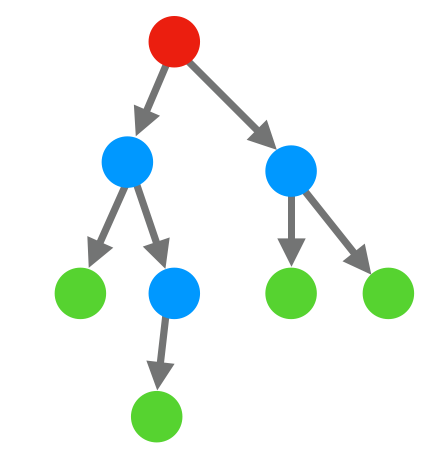
\includegraphics[scale = 0.3]{./images/baum.png}
	\label{2.baum.image}
    \caption{gewurzelter Baum}
	\end{center}
\end{figure}
Bäume sind Grundlage unteranderen des hierarchischen Datenbankmodells, welches sich dadurch auszeichnet, dass jeder Knoten nur einen Vorgänger haben kann.
Dieses Datenbankmodell hat den Nachteil, dass bedingt durch die Kreisfreiheit eines Baumes sehr eingeschränkt ist und beispielsweise keine n:n Beziehungen modelliert werden können.
Das Netzwerkdatenbankmodell versucht dieses Problem zu lösen, indem die Limitierung auf einen Vorfahren aufgehoben wird \cite{hald2013datenbank}.